\newpage
%\addtolength{\parskip}{0.25cm}
%\newpage

\addtolength{\parskip}{0.25cm}

\vspace{2ex}
\noindent
{\large \textbf{Appendix A: Detailed Algorithms}}
\label{sec-apd-algorithms}

\noindent
{\textbf{1. Procedure \rgraphsim (Section~\ref{sec-tsimAlg})}}

\vspace{-2ex}
\begin{figure}[h!]
%\vspace{-2ex}
\begin{center}
{\small
\myhrule
\vspace{-2ex}
\mat{0ex}{
\sstab {\sl Input:\/} Pattern graph $P(V_{P}, E_{P})$ and ball $\ball{[v, r]}$.\\
{\sl Output:\/} The match graph $G_s$ for $P$ in $\ball{[v, r]}$ .\\
\sstab \bcc \hspace{1ex} \= \For each $u \in V_{P}$ \Do\\
\icc \>\hspace{2ex}\= $\matchs(u)$ := \{$w | w$ is in $\ball{[v, r]}$ and $l_P(u)\in l(w)$\};\\
\icc \> \While there are changes \Do\\
\icc \>\> \For each edge ($u, u'$) in $E_P$ and each node $w \in \matchs(u)$ \Do\\
\icc \>\>\hspace{2ex}\= \If there is no edge ($w, w'$) in $\ball{[v, r]}$ with $w' \in \matchs(u')$ \Then\\
\icc \>\>\>\hspace{2ex}\= $\matchs(u)$ := $\matchs(u) \setminus \{w\}$;\\
\icc \>\> \If $\matchs(u)$ = $\emptyset$ \Then \Return $\emptyset$;\\
\icc \> $\Reps$ := \{$(u,w) | u \in V_{P}, w \in \matchs(u)$\};\\
\icc \> Construct the match graph $G_s$ \wrt $\Reps$;\\
\icc \> \Return $G_s$;\\
}

\vspace{-5.5ex} \myhrule
}
\end{center}
\vspace{-4ex}
\caption{Procedure \rgraphsim} \label{alg-rsim}
\vspace{-2ex}
\end{figure}

As shown in Fig~\ref{alg-rsim}, given $P$ and ball $\ball{[v, r]}$,
\rgraphsim finds the match graph for $P$ in $\ball{[v, r]}$.
For each node $u$ in $V_{P}$, it first computes the set $\matchs(u)$ of candidate matches $w$ containing the label of $u$ (lines 1-2),
and then removes nodes from $\matchs(u)$ iteratively (lines 3-7).
A node $w$ is removed from $\matchs(u)$ if there is an adjacent node $u'$ of $u$,
but there exists no adjacent node $w'$ of $w$ such that $w'\in \matchs(u')$.
If so, \rgraphsim constructs the match graph $G_s$ \wrt the maximum match relation $\Reps$ and returns it (lines 8-10).

\eat{%%EAT
\noindent
{\textbf{2. Algorithm \minp (Section~\ref{subsec-batch-opt})}}

\vspace{-2ex}
\begin{figure}[h!]
%\vspace{-2ex}
\begin{center}
{\small
\myhrule \vspace{-2ex}
\mat{0ex}{
\sstab {\sl Input:\/} Pattern graph $P(V_P$, $E_P)$.\\
{\sl Output:\/} A minimum equivalent pattern graph $P_m$ of $P$.\\
\sstab \bcc \hspace{1ex}\= \If $P$ is not a satisfiable pattern graph \Then \Return \bf{null}.\\
\icc \> Compute the maximum match relation $\Reps$ of $P \eps P$;\\
\icc \> Compute equivalent classes of nodes in $P$ based on $\Reps$;\\
\icc \> Create a node for each equivalent class in $P_m$;\\
\icc \> Connect different equivalent classes by necessary edges in $P_m$;\\
\icc \> Compute the intersection of capacity bounds on nodes in each\\
\>\hspace{0.5ex} equivalent class and put on the node in $P_m$;\\
\icc \> \Return $P_m$;\\
}
\vspace{-6ex}

\myhrule
}
\end{center}
\vspace{-4ex}
\caption{Algorithm \minp} \label{alg-minp}
\vspace{-2ex}
\end{figure}

As shown in Fig.~\ref{alg-minp}, given a pattern $P$, \minp returns a minimum equivalent pattern $P_m$ of $P$.
It firstly checks to see whether $P$ is satisfiable (line 1).
If so, it computes the maximum match relation $\Reps$ by treating $P$ as both pattern and data graph via graph simulation (line 2),
and then computes equivalent classes for nodes in $P$ such that $u$ and $w$ are in the same class iff both $(u, w)\in \Reps$ and $(w, u)\in \Reps$(line 3).
It constructs $P_m$ (lines 4-6) by
(a) creating a class node for $P_m$ for each equivalent class,
(b) connecting the class nodes for $P_m$ iff there exist edges in $P$ connecting two pattern nodes which belong to two equivalent classes, and
(c) computing the intersection of capacity bounds on pattern nodes in each equivalent class and put on the corresponding class node in $P_m$.
\looseness=-1

\vspace{-2ex}
\etitle{Correctness \& Complexity}. The correctness of \minp is assured by following.
(1) The maximum match relations returned by $P$ and $P_{m}$ on any data graph $G$ are always same via graph simulation.
(2) The generated capacity bound on each node in $P_{m}$ assures that, the matched nodes of $P_{m}$ in $G$ always satisfy all capacity bounds on the nodes in $P$, which are in the same equivalent class.
Till now, $P\equiv P_{m}$;
(3) For any $P'$ that $P'\equiv P_{m}$, $|P_{m}|\leq|P'|$.
Algorithm \minp is in $O(|P|^2)$ time, by the time complexity of graph simulation.
}%%%EAT

\noindent
{\textbf{2. Algorithm \kw{PFrag} (Section~\ref{sec-dynamictopk})}}

\kw{PFrag} works by connecting the {\em pattern fragmentation} problem to the
{\sc $(k, \nu)$-Balanced Partition} problem.
It is to divide the nodes of a graph into $k$ components such that each component is of size no more than $\nu\cdot\frac{|V|}{k}$, and the number of edges between different components is minimized.
As illustrated before, the $(k,\nu)$-balanced partition problem,
though is not approximable in general, has a number of sophisticated heuristic algorithms~\cite{AndreevR06}.

\vspace{-2ex}
\begin{figure}[h!]
\begin{center}
{\small
\begin{center}
\myhrule \vspace{-2ex}
\mat{0ex}{
\sstab {\sl Input:\/} \= Pattern graph $P(V_{P},E_{P})$ and integer $h$.\\
{\sl Output:\/} An $h$-fragmentation \{${P}_{f1}$, \ldots, ${P}_{fh}$, $C$\} of $P$.\\
\sstab \bcc \hspace{0.5ex} \= $k$ := $h$; $\nu$ := $h$; $M_P$ := $|P|$; $M_C$ := 0;\\
\icc \> $({P}^\nu_{f1}, \ldots, {P}^\nu_{fh}, C^\nu)$ := $\kw{BalanceP}(k,\nu)$; \\
\icc \> $M^\nu_P$ := $\kw{max}\{|{P}^\nu_{f1}|, \ldots, |{P}^\nu_{fh}|\}$; $M^\nu_C$ := $|C^\nu|$;\\
\icc\> \While $\kw{max}\{M_P, M_C\} > \kw{max}\{M^\nu_P, M^\nu_C\}$ \Do\\
\icc \>\hspace{2ex}\= ${P}_{f1}$ := ${P}^\nu_{f1}$, \ldots, ${P}_{fh}$ := ${P}^\nu_{fh}$;\\
\icc \>\hspace{2ex}\= $C$ := $C^\nu$; $M_P$ := $M^\nu_P$; $M_C$ := $M^\nu_C$;\\
\icc \>\> \If $M^\nu_P \geq M^\nu_C$ \Then $\nu := \frac{\nu}{2}$ \Else $\nu := \frac{3\nu}{2}$;\\
\icc \>\> $({P}^\nu_{f1}, \ldots, {P}^\nu_{fh}, C)$ := $\kw{BalanceP}(k,\nu)$;\\
\icc \>\> $M^\nu_P$ := $\kw{max}\{|{P}^\nu_{f1}|, \ldots, |{P}^\nu_{fh}|\}$; $M^\nu_C$ := $|C^\nu|$;\\
\icc \> \Return \{${P}_{f1}$, \ldots, ${P}_{fh}$, $C$\};
}
\vspace{-2.5ex} \myhrule
\end{center}
}
\end{center}
\vspace{-4ex}
\caption{Algorithm \kw{PFrag} \label{alg-pfrag}}
\vspace{-2ex}
\end{figure}

As shown in Fig.~\ref{alg-pfrag}, given $P$ and integer $h$,
\kw{PFrag} finds an $h$-fragmentation for $P$ by recursively invoking algorithm $\kw{BalanceP}(k,\nu)$ for the {\sc $(k,\nu)$-Balanced partition} problem ($\nu\geq 1$) with different $\nu$,
such that the final returned $h$-fragmentation strikes a balance between the size of each fragment ${P}_{fi}$ and the size of the cut $C$.
More specifically, \kw{PFrag} maintains $M_P$ and $M_C$ as the size of the largest fragment ${P}_{fi}$ and the size of the cut respectively.
Initially, it sets $M_P$ to $|P|$ and $M_C$ to 0 (line~1).
It then invokes \kw{BalanceP} with both $k$ and $\nu$ being $h$, \ie has no constraints on the size of fragments of $P$ (line~2).
After that, it iteratively checks whether the generated $h$-fragmentation can be improved (line~4) by adjusting $\nu$ in a {\em binary search style} (lines~4-9).
If the current size $M^\nu_P$ of the largest fragment is no smaller than the size $M^\nu_C$ of the cut,
it invokes \kw{BalanceP} with $h$ and $\frac{\nu}{2}$, or with $h$ and $\frac{3\nu}{2}$ otherwise (line~7).
It returns the $h$-fragmentation if it cannot be improved anymore (line~10).

\vspace{-1.5ex}
\etitle{Correctness \& Complexity}.
The correctness is obvious as \kw{PFrag} always returns an $h$-fragmentation.
Algorithm~\kw{PFrag} runs in $O(\log h\cdot t_{\kw{BalanceP}})$, where $t_{\kw{BalanceP}}$ is the complexity of the algorithm for the {\sc $(k,\nu)$-Balanced Partition} problem. Indeed, \kw{PFrag} calls at most $\log h$ times \kw{BalanceP}, as $\nu\geq 1$.
\looseness=-1


\vspace{1ex}
\noindent
{\large \textbf{Appendix B: Detailed Proofs}}
\label{sec-apd-proofs}

\noindent
{\textbf{1. Proof of Proposition~\ref{prop-pattern-consistency}}}

We will prove the proposition by providing the $O(|P|^2)$ time algorithm, along with its correctness proof.

\vspace{-1.5ex}
The satisfiability of patterns $P$ can be checked by the following algorithm:
(a) Compute the maximum match relation $\Reps$ of $P \eps P$;
(b) Check for each $(u, v)\in \Reps$ with the capacity bounds $[x_u, y_u]$ on $u$ and $[x_v, y_v]$ on $v$, respectively, whether $x_v \leq y_u$ holds.
One can verify that step (a) is in $O(|P|^2)$ time by invoking procedure \rgraphsim; and step (b) can be checked in $O(|P|^2)$ time as the size of $M$ is bounded by $|P|^2$. Thus the algorithm is overall in $O(|P|^2)$ time.

\vspace{-1.5ex}
We next prove the correctness of the algorithm.

\vspace{-1.5ex}
(I) We firstly prove that when the algorithm outputs ``yes", then pattern $P$ is indeed satisfiable.
This is correct since if the algorithm outputs ``yes", \ie $P \eps P$ \wrt $\Reps$ and capacity bounds in $\Reps$ are satisfied, there must exist a data graph $G$ such that $P \eeps G$.
$G$ can be derived by (i) computing equivalent classes of nodes in $P$ based on $\Reps$, such that $u$ and $w$ are in the same class iff both $(u, w)\in \Reps$ and $(w, u)\in \Reps$;
(ii) creating a set of nodes for each equivalent class, where the cardinality of the set falls in the intersection of capacity bounds on nodes in the equivalent class; and
(iii) connecting the nodes belong to two equivalent classes iff there exist edges in $P$ connecting two pattern nodes which belong to the same two equivalent classes.
We also set $r$ to be the radius of $G$. One can verify that $P \eeps G$.

\begin{figure*}[tb!]
	%\begin{widepage}
	\vspace{-1.5ex}
	\begin{center}
		\hspace{-8ex}
		\begin{minipage}[t]{0.4\textwidth}
			\vspace{2ex}
			\begin{center}
				\subfigure[{Unit data update}]{\label{fig-inc-complexity-data}
					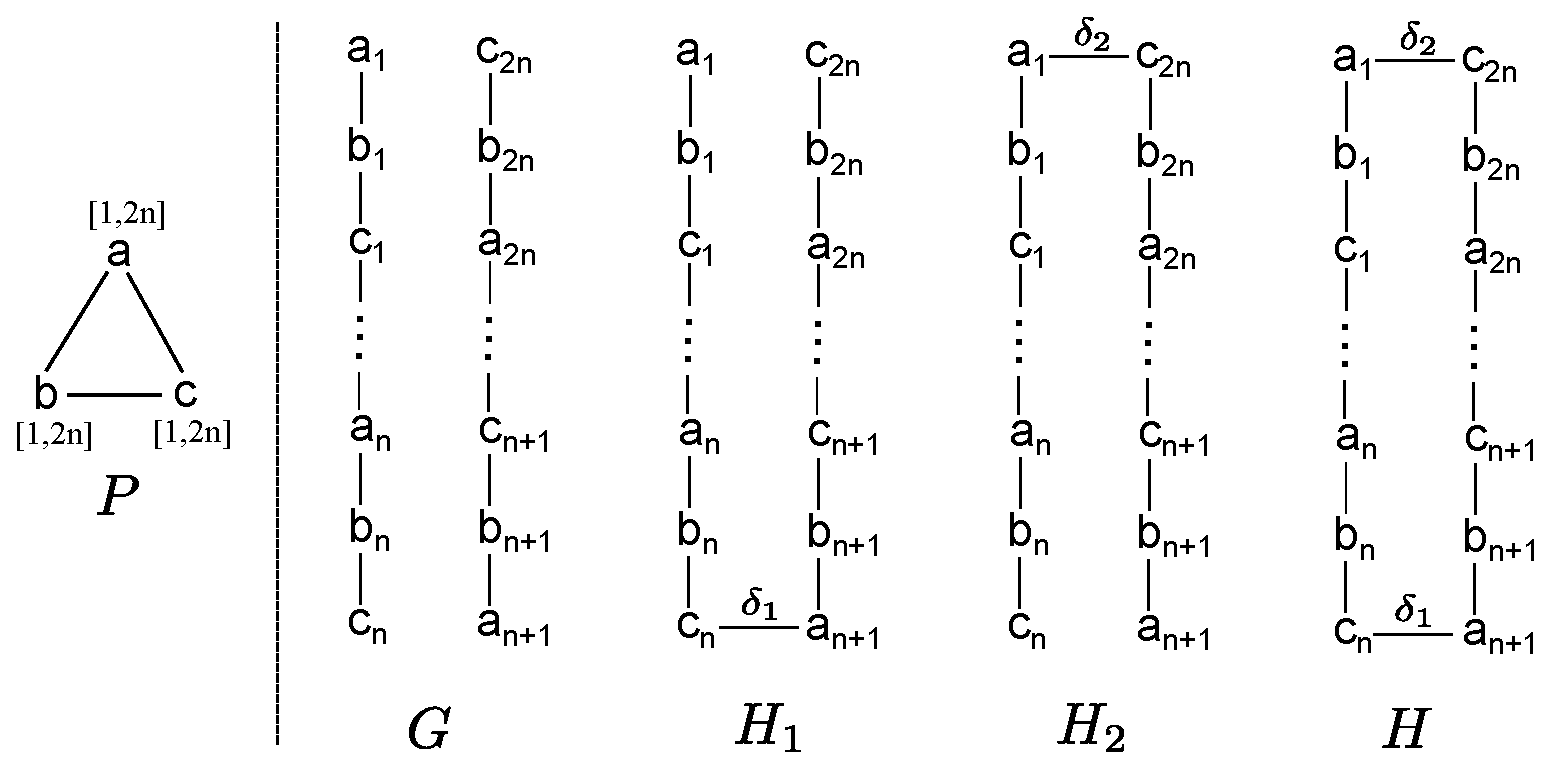
\includegraphics[scale=0.31]{./fig/inc-complexity-proof-data.eps}}
			\end{center}
			\vspace{-2.5ex}
		\end{minipage}
		\hspace{20ex}
		\begin{minipage}[t]{0.4\textwidth}
			\vspace{-0.6ex}
			\begin{center}
				\subfigure[{Unit pattern update}]{\label{fig-inc-complexity-pattern}
					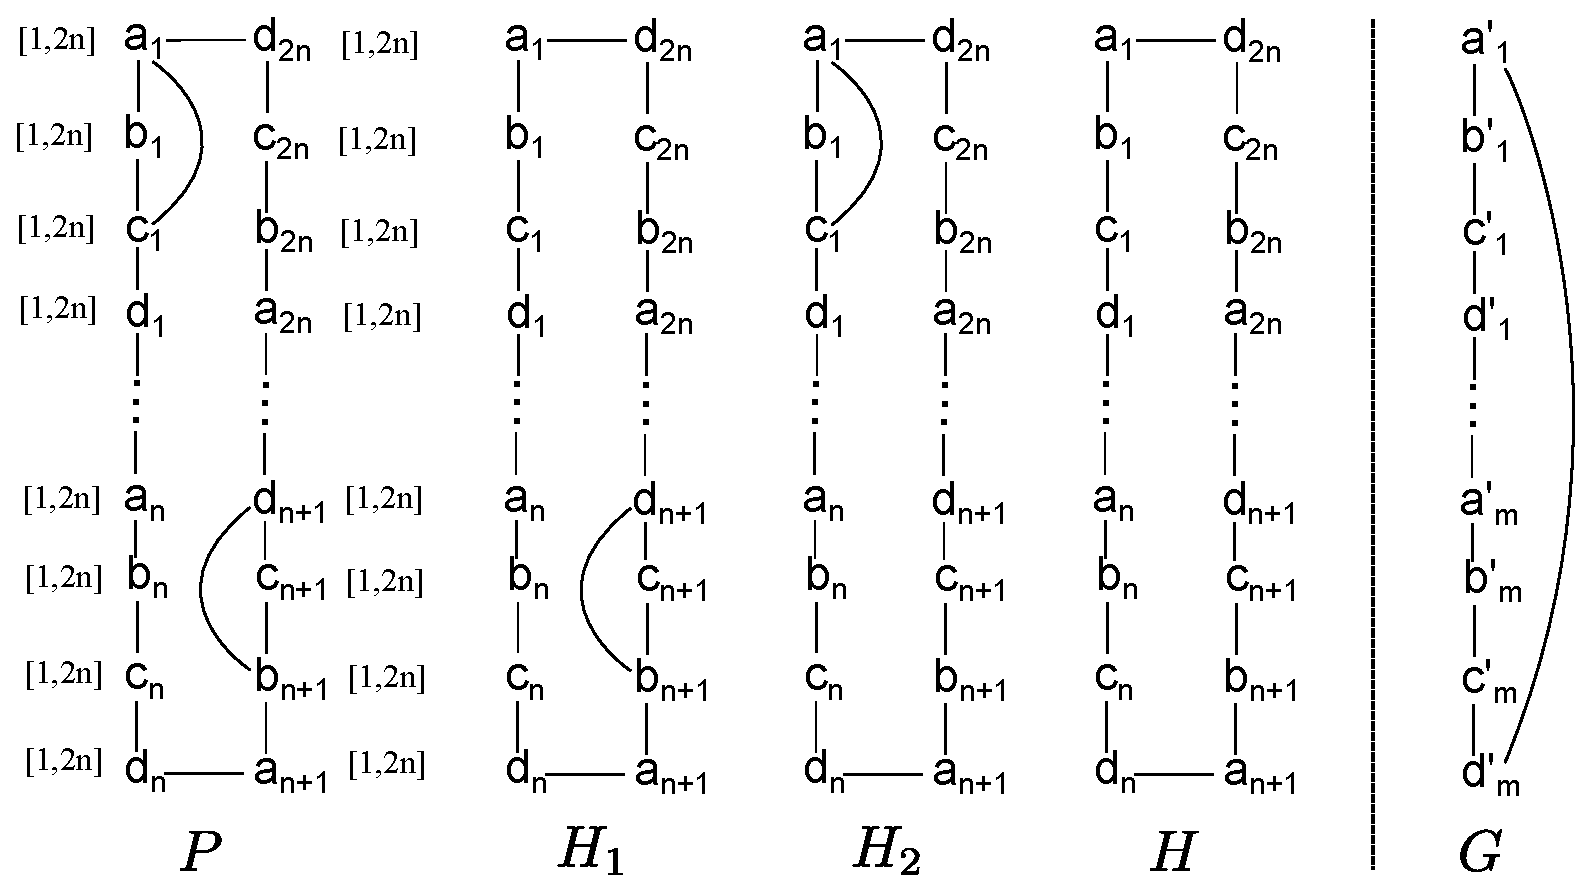
\includegraphics[scale=0.29]{./fig/inc-complexity-proof-pattern.eps}}
			\end{center}
			\vspace{-2.5ex}
		\end{minipage}
	\end{center}
	\vspace{-4ex}
	\caption{Unboundedness of unit data and pattern update}
	\label{proof-patdata-inc}
	%\end{widepage}
	\vspace{-3.0ex}
\end{figure*}

\vspace{-1.5ex}
(II) We then prove that when the algorithm outputs ``no", then pattern $P$ is unsatisfiable.
If the algorithm outputs ``no", then either (i) $P \not\eps P$ or (ii) $P \eps P$ but capacity bounds are not satisfied.
We will prove this by contradiction.
We consider case (i) $P \not\eps P$ and assume that $P$ is satisfiable.
For convenience, we use $P_1 \not\eps P_2$ to denote $P \not\eps P$, while $P_1$, $P_2$ and $P$ are exactly same.
From that $P$ is satisfiable, we know that there exists a data graph $G$ such that $P_1 \eeps G$, $P_2 \eeps G$ and $P_1 \eeps G_s$, where $G_s$ is the perfect subgraph in $G$.
By the definition of team simulation and graph simulation, from $P_2 \eeps G$, we know that $G_s \eps P_2$;
from $P_1 \eeps G_s$, we know that $P_1 \eps G_s$; and 
from $P_1 \eps G_s$ and  $G_s \eps P_2$, we know that $P_1 \eps P_2$.
This contradicts the assumption.
We then consider case (ii), $P \eps P$ \wrt $\Reps$ while there exists $(u, v)\in \Reps$ with the capacity bounds $[x_u, y_u]$ on $u$ and $[x_v, y_v]$ on $v$, respectively, and $x_v > y_u$, and assume that $P$ is satisfiable.
From $P$ is satisfiable, we know that there exists a data graph $G$ such that $P \eeps G$.
From $P \eps P$ \wrt $\Reps$ and $(u, v)\in \Reps$, we know that for any nodes $w$ in $G$, if $w$ matches the pattern node $v$, then it must match the pattern node $u$, that is, the number of data nodes match $u$ is larger than that of data nodes match $v$.
However, this contradicts that the upper bound of $u$ ($y_u$) is smaller than the lower bound of $v$ ($x_v$).
%From (I) and (II) the correctness of the algorithm follows.


\noindent
{\textbf{2. Proof of Theorem~\ref{thm-tsim-radius}}}

We will prove Theorem~\ref{thm-tsim-radius} (1) firstly.
We know that $P\eps \ball{[v, t]}$, and suppose that $M_t$ is the maximum match relation for $P$ in $\ball{[v, t]}$.
Since $\ball{[v, t]}$ is a subgraph of $\ball{[v, r]}$, 
there must exist a binary relation $M_r$ such that for any $(u, v) \in M_t$, where $u$ is a pattern node and $v$ is the matched data node of $u$ in $\ball{[v, t]}$, 
$(u, v) \in M_r$ holds, where $v$ is the matched data node of $u$ in $\ball{[v, r]}$, \ie $M_t \subset M_r$.
Since $M_t$ is the maximum match relation for $P$ in $\ball{[v, t]}$ and $M_t \subset M_r$, by the definition of graph simulation, then $P\eps \ball{[v, r]}$ and $M_r$ is a match relation for $P$ in $\ball{[v, r]}$.	

\vspace{-1ex}	
We will prove Theorem (2) using the lemma below. 

\vspace{-2.7ex}
\begin{lemma}
	\label{lemma-innerball}
	For any data graphs $G_1$ and $G_2$, and pattern graph $P$, if $G_1$ is a subgraph of $G_2$,
	then $M_1 \subset M_2$, where $M_i$ $(i=1,2)$ is the maximum match relation for $P$ in $G_i$ via graph simulation. 
\end{lemma}
\vspace{-2.5ex}

We next prove the lemma and then use the lemma to prove Theorem~\ref{thm-tsim-radius} (2).

\vspace{-1.3ex}
\stitle{Proof of Lemma~\ref{lemma-innerball}:} We will prove the lemma by contradiction. 
We know that $G_1$ is a subgraph of $G_2$, and suppose $M_1 \not\subset M_2$.
That is, there exists a pair of nodes $(u, v) \in M_1$, where $u$ is a pattern node 
and $v$ is the matched data node of $u$, but $(u, v) \not\in M_2$.
By the definition of graph simulation, from $(u, v) \in M_1$, we know that for any child node $u'$ of $u$ in $P$,
there exists a child node $v'$ of $v$ in $G_1$ such that $(u', v') \in M_1$.
From $(u, v) \not\in M_2$, we know that there exists a child node $u''$ of $u$ in $P$, 
but there exist no child nodes $v''$ of $v$ in $G_2$, such that $(u'', v'') \eps M_2$.
The process to compute maximum match relations for graph simulation is a recursive process to 
remove unmatched nodes from the initialized match relations $M$.
Because there exist no $u''$ in $G_2$ such that $(u'', v'') \eps M_2$, $(u, v)$ is removed from $M_2$.
Since $G_1$ is a subgraph of $G_2$, $(u, v)$ should also be removed from $M_1$, 
such that $(u, v) \not\in M_1$.
This contradicts the assumption that $(u, v) \in M_1$, and we get the lemma proved.
\eop

\vspace{-1.5ex}
By Lemma~\ref{lemma-innerball}, since $\ball{[v, t]}$ is a subgraph of $\ball{[v, r]}$, then $M' \subset M$.
By the definition of match graphs, since $M' \subset M$, then $G'_s$ is a subgraph of $G_s$.


\noindent
{\textbf{3. Proof of Proposition~\ref{thm-inc-grouprec-pat}}}

Incremental complexity is defined in terms of LP (locally persistent) graph algorithms \cite{Reps96}.
We also adopt the notion to prove unboundedness of graph algorithms for \dynteamF.

\vspace{-1.5ex}
The proofs below strictly follows the one in \cite{Reps96}.

%\vspace{-1.5ex}
%\begin{figure}[h]
%	\label{fig-inc-complexity-data}
%	\begin{center}
%		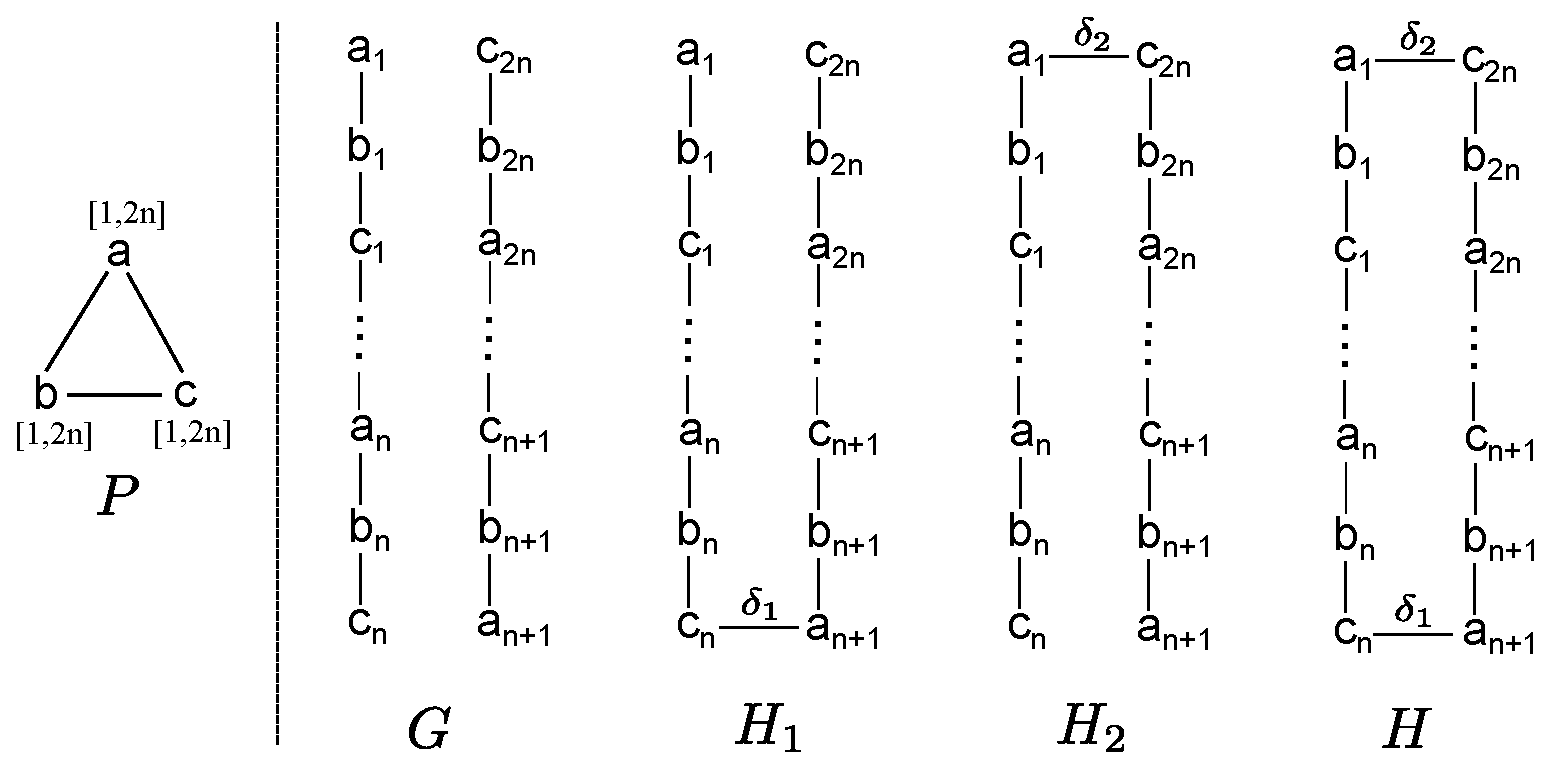
\includegraphics[scale=0.3]{./fig/inc-complexity-proof-data.eps}
%	\end{center}
%	\vspace{-3ex}
%	\caption{Unboundedness of unit data update}
%	\vspace{-2ex}
%\end{figure}

\vspace{-1.5ex}
\etitle{(I) \dynteamF\, is unbounded for unit data update}.
%Following \cite{Reps96, FanWW13-tods},
Consider the following pattern and data graph, and unit data updates, as shown in Fig.~\ref{proof-patdata-inc} (a).
Let data graph $G$ consist of two chains ($a_1$, $b_1$, $c_1$, \ldots, $a_n$, $b_n$, $c_n$) and ($a_{n+1}$, $b_{n+1}$, $c_{n+1}$, \ldots, $a_{2n}$, $b_{2n}$, $c_{2n}$) where $a_i$, $b_i$ and $c_i$ have labels $A$, $B$ and $C$ respectively.
Let pattern graph be a triangle with nodes $a$, $b$ and $c$ with labels $A$, $B$ and $C$ respectively.
Consider two unit edge insertions $\delta_1$ = $(c_n$, $a_{n+1})^+$ and $\delta_2$ = $(c_{2n}$, $a_1)^+$,
and set $k = 1$ and $r$ = $6n$.
Let $H_1$ and $H_2$ denote the graphs $G\oplus \delta_1$ and $G\oplus \delta_2$, respectively.
Obviously, $L_{k}(P, G) = L_{k}(P, H_1) = L_{k}(P, H_2) = \emptyset$,
while $L_{k}(P, H_1\oplus \delta_2) \neq \emptyset$.
Assume that there exists a locally persistent incremental algorithm ${\cal A}$ for \dynteamF.
Let $Trace(G', \delta')$ denote the sequence of steps executed by ${\cal A}$ in processing some update $\delta'$ to some graph $G'$.
Now consider the following two instances: the application of update $\delta_2$ to $G$ and the application of update $\delta_2$ to graph $H_1$.
Obviously, the update process must behave differently in these two cases, and $Trace(G, \delta_2)$ must be different from $Trace(H_1, \delta_2)$
(because many nodes of $H_1\oplus \delta_2$ are affected, while no node in $G\oplus \delta_2$ is affected).
Since a locally persistent algorithm makes no use of global storage, this can happen only both $Trace(G, \delta_2)$ and $Trace(H_1, \delta_2)$ include a visit to some node $w$ that contains different information in the graphs $G$ and $H_1$.
However, $H_1$ was obtained from $G$ by applying update $\delta_1$.
Hence the information at node $w$ must have been changed during the updating of applying $\delta_1$ to $G$.
Therefore, $Trace(G, \delta_1)$ must also contain a visit to node $w$.
As a characteristic of locally persistent algorithms is that if a node $w$ is visited during the updating of applying change $\delta'$ to graph $G'$,
then every node on some path in $G'$ from a modified node of $\delta'$ to $w$ must have been visited.
Therefore, $Trace(G, \delta_1)$ and $Trace(G, \delta_2)$ both contain a visit to $w$,
from the nodes in $\delta_1$ and $\delta_2$, respectively.
Thus, $Trace(G, \delta_1)$ and $Trace(G, \delta_2)$ include visits to every node on the path from $c_n$ or $a_{n+1}$ to $c_{2n}$ or $a_1$ respectively.
Hence, the time taken for processing update $\delta_1$ to $G$ plus the time taken for processing update $\delta_2$ to $G$ must be no smaller than the distance between $c_n$ or $a_{n+1}$ to $c_{2n}$ or $a_1$, \ie $n$, which is not a constant.
However, $|\kw{AFF}|$ in both cases are 1, such that the complexity of the incremental algorithm ${\cal A}$ cannot be measured by a function of $|\kw{AFF}|$.
Thus, ${\cal A}$ is not a bounded locally persistent incremental algorithm.
%which contradicts the assumption.

\vspace{-1.0ex}
That is, \dynteamF\, is unbounded even for $k=1$ and unit data update.
\looseness=-1

%\vspace{-1ex}
%\begin{figure}[h!]
%	\label{fig-inc-complexity-pattern}
%	\begin{center}
%		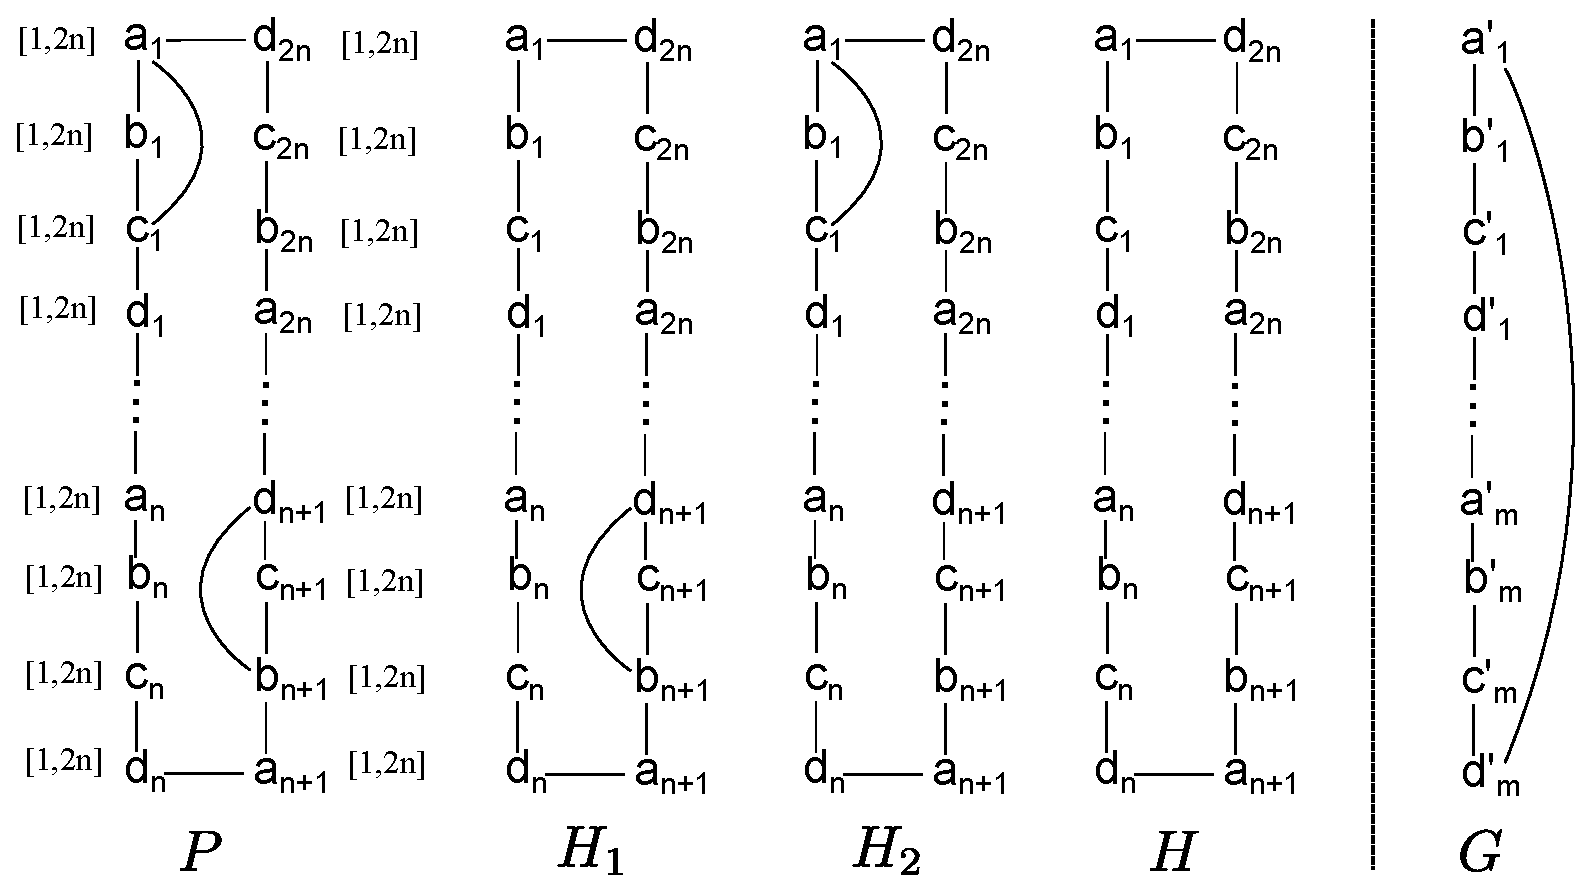
\includegraphics[scale=0.3]{./fig/inc-complexity-proof-pattern.eps}
%	\end{center}
%	\vspace{-3ex}
%	\caption{Unboundedness of unit pattern update}
%	\vspace{-2ex}
%\end{figure}

\vspace{-1.5ex}
\etitle{(II) \dynteamF\, is unbounded for unit pattern update}.
Consider the following pattern and data graph, and unit pattern updates, as shown in Fig.~\ref{proof-patdata-inc} (b).
Let data graph $G$ be a cycle ($a'_1$, $b'_1$, $c'_1$, $d'_1$, \ldots, $a'_m$, $b'_m$, $c'_m$, $d'_m$, $a'_1$),
where $a'_i$, $b'_i$, $c'_i$ and $d'_i$ have labels $A$, $B$, $C$ and $D$ respectively.
Let pattern graph be a cycle ($a_1$, $b_1$, $c_1$, $d_1$, \ldots, $a_n$, $b_n$, $c_n$, $d_n$, $a_{n+1}$, $b_{n+1}$, $c_{n+1}$, $d_{n+1}$, \ldots, $a_{2n}$, $b_{2n}$, $c_{2n}$, $d_{2n}$, $a_1$) and two extra edges ($a_1$, $c_1$) and ($b_{n+1}$, $d_{n+1}$),
where $a_i$, $b_i$, $c_i$ and $d_i$ have labels $A$, $B$, $C$ and $D$ respectively.
Consider two unit edge deletions $\delta_1$ = $(a_1$, $c_1)^-$ and $\delta_2$ = $(b_{n+1}$, $d_{n+1})^-$,
and set $k = 1$ and $r$ = $4m$.
Let $H_1$ and $H_2$ denote the graphs $P\oplus \delta_1$ and $P\oplus \delta_2$, respectively.
Obviously, $L_{k}(P, G) = L_{k}(H_1, G) = L_{k}(H_2, G) = \emptyset$,
while $L_{k}(H_1\oplus \delta_2, G) \neq \emptyset$.
Assume there exists a locally persistent incremental algorithm ${\cal A}$ for \dynteamF.
Let $Trace(P', \delta')$ denote the sequence of steps executed by ${\cal A}$ in processing some update $\delta'$ to some pattern $P'$.
Now consider two instances: the application of update $\delta_2$ to $P$ and the application of update $\delta_2$ to $H_1$.
Obviously, the update process must behave differently in these two cases, and $Trace(P, \delta_2)$ must be different from $Trace(H_1, \delta_2)$
(because many nodes in $G$ for $H_1\oplus \delta_2$ are affected, while no node in $G$ for $P\oplus \delta_2$ is affected).
Since a locally persistent algorithm makes no use of global storage,
this can happen only both $Trace(P, \delta_2)$ and $Trace(H_1, \delta_2)$ include a visit to some node $w$ that contains different information in $P$ and $H_1$.
However, $H_1$ was obtained from $P$ by applying $\delta_1$.
Hence the information at node $w$ must have been changed during the updating of applying $\delta_1$ to $P$.
Therefore, $Trace(P, \delta_1)$ must also contain a visit to node $w$.
%As a characteristic of locally persistent algorithms is that if a node $w$ is visited during the updating of applying update $\delta'$ to pattern $P'$,
%then every node in some path in $P'$ from a modified node of $\delta'$ to $w$ must have been visited.
According to the characteristics of locally persistent algorithms as illustrated in the data updates case,
$Trace(P, \delta_1)$ and $Trace(P, \delta_2)$ both contain a visit to $w$,
from the nodes in $\delta_1$ and $\delta_2$, respectively.
Thus, $Trace(P, \delta_1)$ and $Trace(P, \delta_2)$ include visits to every node on the path from $a_1$ or $c_1$ to $b_{n+1}$ or $d_{n+1}$ respectively.
Hence, the time taken for processing $\delta_1$ to $P$ plus the time taken for processing $\delta_2$ to $P$ must be no smaller than the distance between $a_1$ or $c_1$ to $b_{n+1}$ or $d_{n+1}$, \ie $4n$, which is not a constant.
However, $|\kw{AFF}|$ in both cases are 1, such that the complexity of algorithm ${\cal A}$ cannot be measured by a function of $|\kw{AFF}|$.
Thus, ${\cal A}$ is not a bounded locally persistent incremental algorithm.
%which contradicts the assumption.
That is, \dynteamF\, is unbounded even for $k=1$ and unit pattern update.

\vspace{-1.0ex}
(1) and (2) together prove that \dynteamF\, is unbounded even for $k=1$ and unit pattern or data update.


\noindent
{\textbf{4. Proof of Theorem~\ref{thm-compose}}}

We will prove the theorem by induction.
Given pattern $P(V_P,E_P)$ and its fragmentation \{${P}_{f1}$, \ldots, ${P}_{fh}$, $C$\},
we use $P^{C}(V_{P^{C}},E_{P^{C}})$ to denote the pattern with $V_{P^{C}}$=$V_P$ and $E_{P^{C}}$=$E_P/C$.
%we use $P^{C}(V_P,E_P/C)$ to denote the pattern with the same node set $V_P$ with $P$, and edges excluding the cut $C$ from $E_P$.
Graph simulation is an iterative process to remove unmatched nodes from the candidate nodes,
as illustrated in procedure \rgraphsim in Fig.~\ref{alg-rsim}.
We utilize $M_{C}^{k}$ (resp. $M_{i}^{k}$, $M^{k}$) to denote the match relation for $P^{C}$ (resp. $P_{fi}$, $P$) in $\ball{}$ in the $kth$ iteration.
By the definition of graph simulation, we have $M_{C}^{k}$ = $\bigcup_{i=1}^{h}M_{i}^{k}$.
To prove $M\subseteq\bigcup_{i=1}^{h}M_{i}$,
we next prove $M^{k}\subseteq M_{C}^{k}$ for each iteration instead.

\vspace{-1.8ex}
\sstab{(1)} For $k=0$, \ie the initialization step of graph simulation algorithm,
the algorithm computes the set of candidate matches for each pattern node.
As $P$ and $P^{C}$ have exactly the same node set, we have $M^{0}= M_{C}^{0}$.

\vspace{-1.8ex}
\sstab{(2)} For $k=n$ $(n\geq 0)$, if $M^{n}\subseteq M_{C}^{n}$ holds, we prove $M^{n+1}\subseteq M_{C}^{n+1}$ holds in the $(n+1)th$ iteration.
Suppose both $(u,w)\in M^{n}$ and $(u,w)\in M_{C}^{n}$ hold,
and in the $(n+1)th$ iteration, $(u,w)$ is removed from $M_{C}^{n}$ if there is an adjacent node $u'$ of $u$ in $P_{C}$,
but there exists no adjacent node $w'$ of $w$ in $G$ such that $(u',w')\in M_{C}^{n}$.
Therefore, $(u,w)$ must be removed from $M^{n}$ as $E_{P^{C}} \subseteq E_{P}$,
that is, the edge $(u,u')$ in $E_{P^{C}}$ must belong to $E_{P}$.
Thus, we have $M^{n+1}\subseteq M_{C}^{n+1}$.

\vspace{-1.5ex}
By (1) and (2), we have proven that $M\subseteq\bigcup_{i=1}^{h}M_{i}$.

\noindent
{\textbf{5. Proof of Proposition~\ref{prop-fragmentation}}}

The decision version of the {\em pattern fragmentation} problem, denoted by $\kw{dOFGP}(P, h, r_1, r_2)$,
is to decide whether there exists a fragmentation \{${P}_{f1}$, \ldots, $P_{fh}$, $C$\} such that,
(a) $\max_i |P_{fi}| \leq r_1\cdot\frac{|P|}{h}$ and (b) $|C|\leq r_2|P|$.

\vspace{-1.5ex}
\etitle{Upper bound.} We show the \NP upper bound by providing an \NP algorithm to determine whether there exists an $h$-fragmentation of $P$.\,Given $P$, the algorithm works as follows.
\looseness=-1

\vspace{-1.8ex}
\sstab{(1)} Guess an $h$-fragmentation ${\cal P}_h$ of $P$.

\vspace{-1.8ex}
\sstab{(2)} Check whether it satisfies restrictions of $r_1$ and $r_2$ (conditions (a) and (b) in the definition of $\kw{dOFGP}$).
If so, return yes, otherwise go to the first step and guess another instance.

\vspace{-1.5ex}
The algorithm is in \NP since step~(2) can be checked in \PTIME (liner time, indeed).

\revise{
\vspace{-1.5ex}
\etitle{Lower bound.}
We next show that it is \NP-hard to determine whether there exists an $h$-fragmentation and remains \NP-hard even when $h$ = 2,
by reduction from the {\em minimum cut} problem, which is known \NP-complete\footnote{\small http://www.nada.kth.se/$\sim$viggo/wwwcompendium/node85.html}.

\vspace{-1ex}
An instance of the minimum cut problem is given an undirected graph $H=(V_{H},E_{H})$ and a positive integer $m$,
to find a set $S \subseteq E_{H}$ of edges whose removal leaves two disjoint connected components, with $|S|\leq m$.

\vspace{-1ex}
Given an instance of the minimum cut problem,
we construct an instance of $h$-fragmentation problem.
It can be achieved by taking $H$ as $P$, and setting $h=2$, $r_1=h$ and $r_2 = m/|P|$.
Indeed, the minimum cut problem is a special case of the of $h$-fragmentation problem.}


\eat{%%%% Wrong proof %%%
\vspace{-2.5ex}
\etitle{Lower bound.}
We next show that it is \NP-hard to determine whether there exists an $h$-fragmentation and remains \NP-hard even when $h$ = 2,
by reduction from the {\em minimum cut} problem, which is known \NP-complete\footnote{\small http://www.nada.kth.se/$\sim$viggo/wwwcompendium/node85.html}.

\vspace{-2ex}
An instance of the minimum cut problem is given an undirected graph $H=(V_{H},E_{H})$ and a positive integer $m$,
to find a set $S \subseteq E_{H}$ of edges whose removal leaves two disjoint connected components, with $|S|\leq m$.

\vspace{-2ex}
Given an instance of the minimum cut problem,
we construct an instance of $h$-fragmentation problem.
It can be achieved by taking $H$ as $P$, and setting $h=2$, $r_1=h$ and $r_2 = m/|P|$.
Indeed, the minimum cut problem is a special case of the of $h$-fragmentation problem.
}%%EAT

\noindent
{\textbf{6. Proof of Proposition~\ref{prop-canaffballs}}}

The proposition is correct as when $\Delta P$ comes, the perfect subgraphs must reside in the balls that match all pattern fragments of $P\oplus \Delta P$.
\identifyaffball identifies \affballsx who already match all fragments of $P$;
Or else, if there exists a fragment $P_{fi}$ of $P$ that an \affballx cannot match,
there must exist an edge/node deletion in $\Delta P$ on $P_{fi}$,
such that the ball may match the updated fragment $P_{fi}\oplus \Delta P$.
Thus, \identifyaffball filters out the balls that cannot not match at least one fragment of $P$, and there are no deletion updates on the fragment.

\noindent
{\textbf{7. Proof of Proposition~\ref{prop-affected-datainc}}}
	
The proof is similar to the one of Proposition~\ref{prop-canaffballs}.
\identifyaffball filters out the balls that cannot match all pattern fragments,	and there are no data updates on the ball.


%%%%%%%%%%%%%%%%%%%%%%%%%%%%%%%%%%%%%%%%%%%%%%%%%
\begin{figure*}[tb!]
	%\begin{widepage}
	%\vspace{-2ex}
	\begin{center}
		%\hspace{-5.5ex}
		\subfigure[{\scriptsize Varying $|V_{P}|$ (\youtube)}]{\label{fig-exp-semantic-youtube-diameter}
			\includegraphics[scale=0.38]{./fig/youtube-semantic-diameter.eps}}
		\hspace{0.2ex}
		\subfigure[{\scriptsize Varying $|V_{P}|$ (\youtube)}]{\label{fig-exp-semantic-youtube-density}
			\includegraphics[scale=0.38]{./fig/youtube-semantic-density.eps}}
		\hspace{0.2ex}
		\subfigure[{\scriptsize Varying $|V_{P}|$ (\youtube)}]{\label{fig-exp-semantic-youtube-capacity}
			\includegraphics[scale=0.38]{./fig/youtube-semantic-capacity.eps}}
		\hspace{0.2ex}
		\subfigure[{\scriptsize Varying $|V_{P}|$ (\youtube)}]{\label{fig-exp-semantic-youtube-link}
			\includegraphics[scale=0.38]{./fig/youtube-semantic-link.eps}}
		\vspace{-2.5ex}
		
		%\hspace{-5.5ex}
		\subfigure[{\scriptsize Varying $k$ (\youtube)}]{\label{fig-exp-semantic-youtube-diameter-varyk}
			\includegraphics[scale=0.38]{./fig/youtube-semantic-diameter-varyk.eps}}
		\hspace{0.2ex}
		\subfigure[{\scriptsize Varying $k$ (\youtube)}]{\label{fig-exp-semantic-youtube-density-varyk}
			\includegraphics[scale=0.38]{./fig/youtube-semantic-density-varyk.eps}}
		\hspace{0.2ex}
		\subfigure[{\scriptsize Varying $k$ (\youtube)}]{\label{fig-exp-semantic-youtube-capacity-varyk}
			\includegraphics[scale=0.38]{./fig/youtube-semantic-capacity-varyk.eps}}
		\hspace{0.2ex}
		\subfigure[{\scriptsize Varying $k$ (\youtube)}]{\label{fig-exp-semantic-youtube-link-varyk}
			\includegraphics[scale=0.38]{./fig/youtube-semantic-link-varyk.eps}}
		\vspace{-2.0ex}
		
	\end{center}
	\vspace{-3.0ex}
	\caption{Performance evaluation of \optgrouprec for top-$k$ team formation problem}
	\label{exp-semantic-effectiveness-youtube}
	%\end{widepage}
	\vspace{-3.0ex}
\end{figure*}


%%%%%%%%%%%%%%%%%%%%%%%%%%%%%%%%%%%%%%%%%%%%%%%%%


\vspace{1ex}
\noindent
{\large \textbf{Appendix C: Detailed Correctness \& Complexity Analysis}}
\label{sec-apd-complexity}

\noindent
{\textbf{1. Algorithm \incp (Section~\ref{subsec-Qinc})}}

The correctness of \incp \wrt $\Delta P$ is assured by
the correctness of (a) \identifyaffball (by Proposition~\ref{prop-canaffballs});
(b) \incmatch, which is assured by the correctness of \rgraphsim that has been proved in Section~\ref{sec-tsimAlg}, and the correctness of of \patedgeinsert. Indeed, \patedgeinsert only removes
nodes that are no longer valid matches in each $M(P_{fi}, \ball{[v,r]})$;
(c) \comb, whose analysis follows the same way as that of \patedgeinsert; and
(d) the early return property (by Lemma~\ref{lemma-approximation-bound}).

\vspace{-1.5ex}
Procedure \identifyaffball runs in $O(2^{h}\cdot(|\Delta P|+h) +||\affballsx||)$ time, where it takes $O(2^{h}\cdot|\Delta P|)$ time to update \bfc, $O(2^{h}\cdot h)$ to do the AND-operation, and $O(||\affballsx||)$ to identify \affballsx.
%Thus, procedure \identifyaffball runs in $O(2^{h}\cdot(|\Delta P|+h) +||\affballsx||)$.
As $h$ is typically small, \eg 2 to 5, thus \identifyaffball is in $O(|\Delta P|+||\affballsx||)$;
\patedgeinsert is in $O(|M(P_{fi}, \ball{[v,r]})|+|V_{P_{fi}}||E_{\ball{[v,r]}}|)$ time.
Indeed, the recursive process for checking invalid nodes in $M(P_{fi}, \ball{[v,r]})$ is bounded by $O(|V_{P_{fi}}||E_{\ball{[v,r]}}|)$,
and the process to update $M(P_{fi}, \ball{[v,r]})$ is bounded by the size of its changes, which is monotonically decreasing;
According to \patedgeinsert,
\comb is in $O(|\bigcup^{h}_{i=1} rM(P_{fi}\oplus\Delta P_{fi},\ball{[v,r]})|+r|V_{P\oplus \Delta P}||E_{\ball{[v,r]}}|)$ time.

\vspace{-1.5ex}
Putting these together, algorithm \incp is in
$O(\bigcup_{\hat{G}\in \affballsx}\bigcup_{i\in[1,h]}(|M(P_{fi}, \hat{G})|+r|M(P_{fi} \oplus \Delta P_{fi}, \hat{G})|) + r|P \oplus \Delta P||\affballsx|$ +$|\Delta P|)$ time \wrt $\Delta P$.


\noindent
{\textbf{2. Algorithm \incd (Section~\ref{subsec-Ginc})}}

The correctness of \incd \wrt $\Delta G$ is assured by the correctness of
\identifyaffball (by Proposition~\ref{prop-affected-datainc}) and procedures \incmatch and \comb,
which can be proved along the same lines as for pattern updates.

\vspace{-1.5ex}
One can verify that \identifyaffball is in $O(|\affballsx| + |\Delta G|)$,
\incmatch for all fragments and all \affballsx is in $O(|P||\affballsx|)$ time, and \comb is in $O(\bigcup_{i\in[1,h]}r|M(P_{fi}, \widehat{G\oplus\Delta G})|$ + $r|V_{P}||E_{\widehat{G\oplus\Delta G}}|)$ time.
Therefore, algorithm \incd is in
$O(\bigcup_{\widehat{G\oplus\Delta G}\in \affballsx} \bigcup_{i\in[1,h]}r|M(P_{fi}, \widehat{G\oplus\Delta G})|+r|P||\affballsx| + |\Delta G|)$ time \wrt $\Delta G$.

\vspace{1ex}
\noindent
{\large \textbf{Appendix D: Extra Experiments}}
\label{sec-apd-exp}

\vspace{-0.5ex}
The experimental results on \youtube are reported here.

\vspace{-1.8ex}
\stitle{Exp-1: Performance of \optgrouprec}. We firstly evaluated the performance of \optgrouprec vs. \mindia, \minsumdis and \denalk on \youtube \wrt four quality measures.
The results are reported in Fig.~\ref{fig-exp-semantic-youtube-diameter} to~\ref{fig-exp-semantic-youtube-link-varyk}.
We find \optgrouprec strikes a balance at capturing the practical requirements.

\vspace{-1.8ex}
\stitle{Exp-2: Efficiency of \inc for one set of updates}. Varying the amount of updates in one update set from 4.5\% to 49.5\% for pattern updates, 2.5\% to 27.5\% (resp. 3\% to 33\%) for data insertions and hybrid data updates (resp. data deletions), and (4.5\%, 2.5\%) to (31.5\%, 17.5\%) for simultaneous pattern and data updates, the results are reported in Fig.~\ref{fig-exp-patinc-del-youtube} to~\ref{fig-exp-hyb-patdata-youtube}.
We find that \inc outperforms \optgrouprec when $\Delta P$, $\Delta G$ and $(\Delta P$, $\Delta G)$ are no more than 36\%, 22.5\% and (27\%, 15\%).
%for hybrid pattern, hybrid data, and simultaneous pattern and data updates.

\vspace{-1.8ex}
\stitle{Exp-3: Efficiency of \inc for continuous sets of updates}. We generated 5 sets of updates,
varying the amount of updates from 4.5\% to 27\% for pattern updates, 2.5\% to 15\% for data updates,
and (4.5\%, 2.5\%) to (22.5\%, 12.5\%) for simultaneous pattern and data updates.
We evaluated the average time took by \inc to process these sets of updates one by one.
The results are reported in Fig.~\ref{fig-exp-patinc-multi-youtube} to~\ref{fig-exp-hyb-datapat-multi-youtube}.
We find \inc outperforms \optgrouprec when changes are no more than 27\%, 10\% and (13.5\%, 7.5\%) for continuous pattern, data and simultaneous updates respectively.

\vspace{-1.8ex}
\stitle{Exp-4: Physical storage of auxiliary structures}. As shown in Fig.~\ref{fig-exp-youtube-extraspace},
it takes 58MB extra space to store all auxiliary structures utilized by \inc on \youtube, which need 114MB space to store itself,
\ie 50.8\% compared with the original dataset.

\begin{figure*}[t!]
	%\begin{widepage}
	%\vspace{-1.5ex}
	\begin{center}
		%\hspace{-5.5ex}
		\subfigure[{\scriptsize Varying $|\Delta P|$ (deletions)}]{\label{fig-exp-patinc-del-youtube}
			\includegraphics[scale=0.38]{./fig/youtube-pattern-deletion.eps}}
		\hspace{0.2ex}
		\subfigure[{\scriptsize Varying $|\Delta P|$ (insertions)}]{\label{fig-exp-patinc-ins-youtube}
			\includegraphics[scale=0.38]{./fig/youtube-pattern-insertion.eps}}
		\hspace{0.2ex}
		\subfigure[{\scriptsize Varying $|\Delta P|$ (capacity)}]{\label{fig-exp-patinc-cap-youtube}
			\includegraphics[scale=0.38]{./fig/youtube-pattern-capchange.eps}}
		\hspace{0.2ex}
		\subfigure[{\scriptsize Varying $|\Delta P|$ (hybrid updates)\hspace{-8.5ex}}]{\label{fig-exp-patinc-hyb-youtube}
			\includegraphics[scale=0.38]{./fig/youtube-pattern-hybrid.eps}}
		\vspace{-2.5ex}
		
		%\hspace{-5.5ex}
		\subfigure[{\scriptsize Varying $|\Delta G|$ (deletions)}]{\label{fig-exp-datainc-del-youtube}
			\includegraphics[scale=0.38]{./fig/youtube-data-deletion.eps}}
		\hspace{0.2ex}
		\subfigure[{\scriptsize Varying $|\Delta G|$ (insertions)}]{\label{fig-exp-datainc-ins-youtube}
			\includegraphics[scale=0.38]{./fig/youtube-data-insertion.eps}}
		\hspace{0.2ex}
		\subfigure[{\scriptsize Varying $|\Delta G|$ (hybrid updates)}\hspace{-5.5ex}]{\label{fig-exp-datainc-hyb-youtube}
			\includegraphics[scale=0.38]{./fig/youtube-data-hybrid.eps}}
		\hspace{0.2ex}
		\subfigure[{\scriptsize Vary $(|\Delta P|,|\Delta G|)$ (simultaneous)}\hspace{-8.5ex}]{\label{fig-exp-hyb-patdata-youtube}
			\includegraphics[scale=0.38]{./fig/youtube-pattern-data.eps}}
		\vspace{-2.5ex}
		
		%\hspace{-5.5ex}
		\subfigure[{\scriptsize Varying $|\Delta P|$ in update sets}]{\label{fig-exp-patinc-multi-youtube}
			\includegraphics[scale=0.38]{./fig/youtube-pattern-multi.eps}}
		\hspace{0.2ex}
		\subfigure[{\scriptsize Varying $|\Delta G|$ in update sets}]{\label{fig-exp-datainc-multi-youtube}
			\includegraphics[scale=0.38]{./fig/youtube-data-multi.eps}}
		\hspace{0.2ex}
		\subfigure[{\scriptsize Vary $(|\Delta P|,|\Delta G|)$ in update sets}\hspace{-8.5ex}]{\label{fig-exp-hyb-datapat-multi-youtube}
			\includegraphics[scale=0.38]{./fig/youtube-pattern-data-multi.eps}}
		\hspace{0.2ex}
		\subfigure[{\scriptsize Storage sizes}]{\label{fig-exp-youtube-extraspace}
			\includegraphics[scale=0.38]{./fig/youtube-space.eps}}
		\vspace{-2ex}
		
	\end{center}
	\vspace{-3.0ex}
	\caption{Performance evaluation of \inc for dynamic top-$k$ team formation problem (\youtube)}
	\label{exp-inc-youtube}
	%\end{widepage}
	\vspace{-3.0ex}
\end{figure*}
